\documentclass{article}

\usepackage{listings}
\usepackage{color}
\usepackage{graphicx}
\usepackage{float}
\usepackage{amsmath}
\usepackage{subfig}
\usepackage{cite}
\usepackage{url}

\begin{document}

\title{Image Analysis - TP2 - Local Filtering and Histograms}

\author{Jander Nascimento, 
\and Raquel Oliveira}

\maketitle

\section{Filtering}
	
	\subsection{Binomial}

		Binomial filter uses Pascal's triangle to create a filter. This filter has the blurry effect with some differences in preserving objects in the image.

One example of a 3x3 Binomial filter can be seen in the Figure \ref{3x3binomial}. The values for this kernel can be obtained from binomial coefficient definition, presented in Equation \ref{equa:bc}.

\begin{equation}
\frac{n!}{(n-k)!k!}={n \choose k}
\label{equa:bc}
\end{equation}

\begin{figure}[H]
  \begin{center}
  \begin{tabular}{ | c | c | c | }
    \hline
    1 & 2 & 1 \\ \hline

    2 & 4 & 2 \\ \hline

    1 & 2 & 1 \\
    \hline
  \end{tabular}
  \end{center}
  \caption{3 x 3 Binomial filter\label{3x3binomial}}\end{figure}

		This kernel is used to remove the noise in image, but it do not preserve the edges of the image. 
		
	\subsection{Median}

		With a purpose of noise reduction, in certain situations Median Filter can preserve the edges while reduce the noise of the image. For this reason this kind of filter is regularly used as a pre-treatment for edge detection.

		The Median filtering differs from others filters in the way it is applied to the image. While other filters are defined by kernels as the aproximation of its derivation, the median filter depends on each sector of the image analyzed to calculate the new pixel intensities.

		Median kernel copies a certain sector of the image analyzed and change the value of the central pixel in the original image. The central pixel in the original image receives the median value of the kernel. It is possible to do it by simply sorting the content of the kernel and assign the value in the middle (central position of the kernel) to the original image. 

	\subsection{Binomial {\it versus} Median}

		\begin{figure}[H]
		  \centering
		  \subfloat[Binomial]{\label{fig:binomial}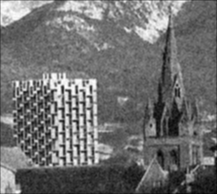
\includegraphics[width=0.4\textwidth]{../image/church_binomial}}                
		  \subfloat[Median]{\label{fig:median}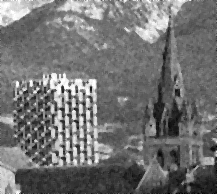
\includegraphics[width=0.4\textwidth]{../image/church_median}}
		  \caption{Removing noise}
		  \label{fig:removingnoise}
		\end{figure}		

	In the Figure \ref{fig:removingnoise} we applied Binomial and Median filter separately. 
	Median preserves the edges better than the Binomial, although the Binomial preserves some central details in the image that the Binomial do not. 
	This behavior can be seen in the window at the chapel, in the Binomial is possible to see the borders of the window more clearly, while in the Median this detail is not displayed at all. 

\section{Histogram}

	The histogram shows the color distribution of a certain image regarding to its color intensity. The 		histogram is represented in a Cartesian, where x axis is the color intensity and y represents the number of pixels that have such intensity.

	In this practical work, we wrote a function in c that computes the intensity histogram. The values are stored in a array of 255 positions. We do not display the histogram as a graph. Just its values are displayed.

	\subsection{Stretching}

	The histogram stretching is a technique by which the color histogram is used to evaluate and possibly change the color intensity range. This enhances the 		detail level of some images that might appear too dark or too bright. This is done by spreading the pixels to use the entire color intensity.
	
	For each pixel of the image, we calculate its new intensity based on the stretching formula:
		\begin{equation}
			y[n]=new_{min}+\frac{new_{max}-new_{min}}{current_{max}-current_{min}}*(x[n]-current_{min})
			\label{eq:stretching}
		\end{equation}
	
		where: 
			\begin{itemize}
	  			\item {\it n} is the pixel		
	  			\item {\it $new_{min}$} is 0;
	  			\item {\it $new_{max}$} is 255; 
				\item {\it $current_{max}$} is the maximum intensity of the color that is used in the image
				\item {\it $current_{min}$} is the minimum intensity of the color that is used in the image
	  			\item {\it x[n]} is the current intensity of the pixel.
			\end{itemize}

	\begin{figure}[H]
	\centering
	\subfloat[Original Image]{\label{fig:original}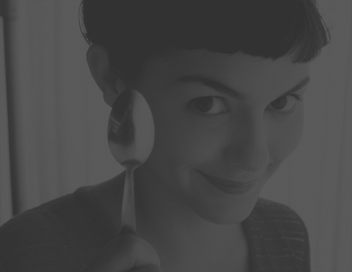
\includegraphics[width=0.3\textwidth]{../image/amelie}}                
	\subfloat[Original Histogram]{\label{fig:orig_histogram}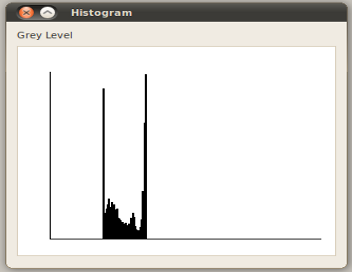
\includegraphics[width=0.3\textwidth]{../image/histogram}}
	\subfloat[Stretched Image]{\label{fig:stretched}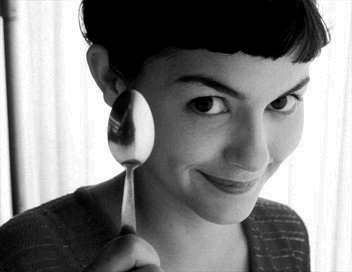
\includegraphics[width=0.3\textwidth]{../image/amelie_stretched}}
	\subfloat[Stretched Histogram]{\label{fig:histogram_s}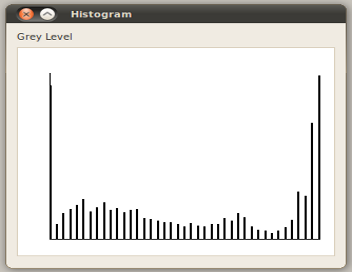
\includegraphics[width=0.3\textwidth]{../image/histogram_stretching}}
	\caption{Stretching Transformation}
	\label{fig:stretching}
	\end{figure}

	\subsection{Equalization}

	Histogram equalization is a method in image processing of contrast adjustment using the image's histogram. This method usually increases the global contrast 		of many images, especially when the usable data of the image is represented by close contrast values. Through this adjustment, the intensities can be better 		distributed on the histogram. This allows for areas of lower local contrast to gain a higher contrast. 

	Based on the histrogram of the image, we compute the cumulative distribution functions, which is the values of the histogram in a cumulative way. For each pixel of the image, we calculate its new intensity based on the equalization formula:
			\begin{equation}
				h[v]= round \left( \frac{cdf(v)-cdf_{min}}{(M * N) - cdf_{min}} * (L-1) \right) 
			\label{eq:equalization}
			\end{equation}
			
			where:		
			\begin{itemize}
	  			\item {\it v} is the current intensity of the pixel		
		  		\item {\it cdf(v)} is the value of such intensity in the array that stores the accumulated values of the histogram
				\item {\it $cdf_{min}$} is the minimum intensity value of the color
		  		\item {\it M} is the height of the image		
		  		\item {\it N} is the width of the image
		  		\item {\it L} is the number of color levels used (in most cases, 256)
			\end{itemize}

	\begin{figure}[H]
	\centering
	\subfloat[Original Image]{\label{fig:original2}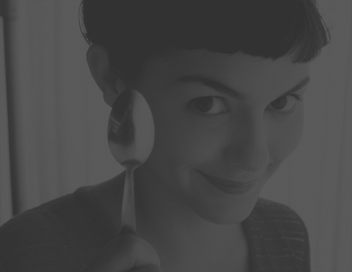
\includegraphics[width=0.3\textwidth]{../image/amelie}}                
	\subfloat[Original Histogram]{\label{fig:orig_histogram2}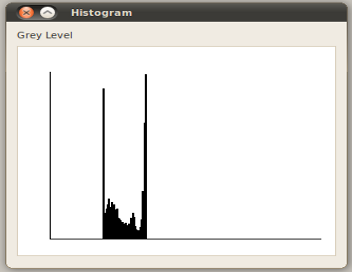
\includegraphics[width=0.3\textwidth]{../image/histogram}}
	\subfloat[Equalized Image]{\label{fig:equalized}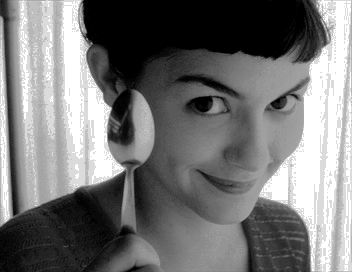
\includegraphics[width=0.3\textwidth]{../image/amelie_equalized}}
	\subfloat[Equalized Histogram]{\label{fig:histogram_e}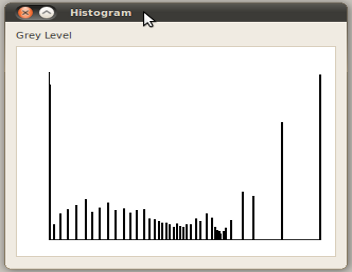
\includegraphics[width=0.3\textwidth]{../image/histogram_equalized}}
	\caption{Equalization Transformation}
	\label{fig:equalizing}
	\end{figure}

	
	\subsection{How to run?}

	Steps to compile the application:
	
	\begin{itemize}
		\item svn checkout https://jfimageanalysis.googlecode.com/svn/trunk/TP2/ \#download source code
		\item make \#compiles the code
	\end{itemize}

	As an input image only {\bf pgm plaintext} files are accepted (P2). 

	Examples of usage:

	\begin{itemize}
		\item Binomial filter to an image:
		\subitem ./imagetransform -f binomial -i image\_in.pgm $>$ image\_out.pgm
		\item Median filter with kernel size {\it s}, applied {\it n} times:
		\subitem ./imagetransform -f median -i image\_in.pgm -s 3 -n 5 $>$ image\_out.pgm
		\item Equalize
		\subitem ./imagetransform -i image\_in.pgm -e $>$ image\_out.pgm
	\end{itemize}

	You can always type {\it ./imagetransform --help} to check for more options. 

\end{document}


